\documentclass[conference]{IEEEtran}
\IEEEoverridecommandlockouts

\usepackage{cite}
\usepackage{amsmath,amssymb,amsfonts}
\usepackage{algorithm}
\usepackage{algpseudocode}
\usepackage{graphicx}
\usepackage{textcomp}
\usepackage{xcolor}
\usepackage{booktabs}
\usepackage{multirow}
\usepackage{tikz}
\usetikzlibrary{arrows.meta,positioning,fit}
\usepackage{url}

\newcommand{\clip}{\operatorname{clip}}
\algrenewcommand\algorithmicrequire{\textbf{Input:}}
\algrenewcommand\algorithmicensure{\textbf{Output:}}

\begin{document}

\title{Twin-in-the-Loop: A Small Language Model Farm Manager Guided by a Learned Plant-Growth Digital Twin}

\author{\IEEEauthorblockN{Rishabh Arya}
\IEEEauthorblockA{\textit{Dept. of Computer Science and Engineering (AI \& ML)}\\
\textit{Dayananda Sagar University}\\
Bengaluru, India\\
rishabharya.k@gmail.com}
\and
\IEEEauthorblockN{Second Author}
\IEEEauthorblockA{\textit{Dept. of Computer Science and Engineering (AI \& ML)}\\
\textit{Dayananda Sagar University}\\
Bengaluru, India\\
second.author@example.com}
\and
\IEEEauthorblockN{Third Author}
\IEEEauthorblockA{\textit{Dept. of Computer Science and Engineering (AI \& ML)}\\
\textit{Dayananda Sagar University}\\
Bengaluru, India\\
third.author@example.com}
}

\maketitle

\begin{abstract}
Digital twins can answer what-if questions about a crop, but someone still has to ask the
right questions and act on the answers. We study whether a small, cheap language model can fill
that role safely. An 8B-parameter open model (Llama~3.1) manages a simulated 144-plant field in
Unity3D for a full season, deciding every three days which of four actuator-limited controls
to change, while unannounced droughts, monsoons, heatwaves and acid rain hit the field. The
model is not told the crop's optimal ranges. A learned plant-growth twin, built from an FAO-56
soil water balance and a calibrated gradient-boosting surrogate, is used twice per decision: to
\emph{probe} how each control would change tomorrow's growth, and to \emph{check} each proposed
action and veto those predicted to do harm. Over 150 seasons in five scenarios, the agent
brings 96\% of seasons to maturity (no intervention: 40\%; a rule-based controller that knows the
true optima: 100\%) at a cost of about \$0.0006 per season. Ablations show that the twin check is
what makes the small model safe: without it, success falls to 52\% and the agent harms even a
calm season. The probes lift acid-soil success from 2/5 to 5/5. A 24B model reaches the same success
with higher crop health and a quarter of the vetoes.
\end{abstract}

\begin{IEEEkeywords}
digital twin, large language model agents, precision agriculture, surrogate model, decision support, Unity3D
\end{IEEEkeywords}

% =============================================================================
\section{Introduction}

Digital twins pair a physical system with a computational model that is updated from it and
used to decide what to do next \cite{grieves2017digital}. In agriculture they promise
what-if analysis for irrigation, soil amendment and climate control
\cite{verdouw2021digital,pylianidis2021introducing}, building on two decades of data-driven
farming \cite{wolfert2017big,liakos2018machine}. A twin answers questions, however; someone
still has to ask the right ones and turn the answers into actions. Large language models
(LLMs) are an obvious candidate for that role: they carry broad agronomic knowledge
\cite{silva2023gpt4,tzachor2023large} and can act as autonomous agents that reason and call
tools \cite{yao2023react,schick2023toolformer,wang2024survey}. They also hallucinate, misread
numbers and contradict themselves, which is unacceptable when an action irrigates a field or
changes its soil chemistry.

This paper studies a deliberately small and cheap configuration: an 8-billion-parameter
open model \cite{grattafiori2024llama3} that manages a simulated 144-plant field for a full
season, while unannounced droughts, monsoons, heatwaves and acid rain hit it. The agent sees the
twin's state but is \emph{not} told the crop's optimal ranges. It makes one LLM call every three
simulated days, with no tool loop and no conversation history, so a season costs well under a
tenth of a US cent. The twin is used twice per decision: before the call, to \emph{probe} how
each control would change tomorrow's growth, and after it, to \emph{check} each proposed action
and veto any that it predicts would do harm.

Our contributions are:
\begin{enumerate}
\item A twin-in-the-loop agent design in which a learned plant-growth twin supplies
one-step what-if probes to the prompt and acts as a safety filter on the reply, under explicit
actuator limits (Section~\ref{sec:agent}).
\item A reproducible benchmark of five weather scenarios with seed-dependent timing and
intensity, a Python replica of the Unity twin tested step-for-step against it, and resilience
metrics per weather event (Section~\ref{sec:setup}).
\item An evaluation over 150 seasons against a no-intervention baseline and a rule-based
controller that knows the true optima, with ablations of the probes, the twin check and the
model size (Section~\ref{sec:results}).
\end{enumerate}

% =============================================================================
\section{Related Work}

\textit{Crop models and digital twins.} Process-based crop models such as DSSAT
\cite{jones2003dssat} and AquaCrop \cite{steduto2009aquacrop} simulate growth from weather,
soil and management, and the FAO-56 guidelines \cite{allen1998fao56} standardise the water
balance most of them share. Verdouw \textit{et al.} \cite{verdouw2021digital} define farm
digital twins by their purpose and level of autonomy, and Pylianidis \textit{et al.}
\cite{pylianidis2021introducing} survey early agricultural twins, most of which stop at
monitoring. gym-DSSAT \cite{gautron2022gymdssat} turns a crop model into a reinforcement
learning environment; reinforcement learning, however, needs many simulated seasons per policy,
while an LLM agent can act from prior knowledge on its first season.

\textit{LLM agents.} ReAct \cite{yao2023react} interleaves reasoning with actions, Toolformer
\cite{schick2023toolformer} learns when to call tools, and Reflexion \cite{shinn2023reflexion}
adds verbal self-feedback across episodes. Grounding is the recurring problem: Huang
\textit{et al.} \cite{huang2022language} show that LLM plans are often not executable, and SayCan
\cite{ahn2022saycan} scores each candidate action with a learned value function before execution.
RAP \cite{hao2023reasoning} lets the LLM plan with a world model. Our twin plays the role of
SayCan's value function and RAP's world model, but with a domain simulator instead of the LLM
itself, and in a single call rather than a search.

\textit{LLMs in agriculture.} GPT-4 passes agronomy exams \cite{silva2023gpt4}, and LLMs are
being considered for extension services \cite{tzachor2023large}. To our knowledge, closed-loop
control of a crop twin by a small open LLM, with the twin as both advisor and safety filter, has
not been evaluated.

% =============================================================================
\section{The Plant-Growth Digital Twin}\label{sec:twin}

The twin simulates a $12\times12$ field of tomato-like plants in Unity3D \cite{juliani2018unity},
each rendered in one of seven growth stages $k\in\{0,\dots,6\}$ (seed to mature). Once per
simulated day it runs a soil water balance, scores the day's growing conditions, and updates
every plant. A Python replica of the same equations is used for batch evaluation; automated
tests check it step for step against the reference implementation, and the C\# surrogate
against parity vectors from it.

\textit{Water balance.} Soil moisture $\theta$ (\% of saturation) is a state. Reference
evapotranspiration follows Turc \cite{turc1961evaluation} with Angstr\"om radiation,
\begin{equation}
\begin{aligned}
ET_0 &= 0.013\,\frac{T}{T+15}\,\bigl(23.8856\,R_s + 50\bigr)\,c_{RH},\\
R_s &= \Bigl(0.25 + 0.5\,\frac{n}{N}\Bigr)R_a,
\end{aligned}
\label{eq:et0}
\end{equation}
where $T$ is air temperature ($^\circ$C), $n$ sunshine hours, $N=12$\,h, $R_a=35$\,MJ\,m$^{-2}$d$^{-1}$
and $c_{RH}=1+(50-RH)/70$ for relative humidity $RH<50\%$ (1 otherwise). Following FAO-56
\cite{allen1998fao56}, crop water use is reduced below the readily available water threshold
$\theta_p=\theta_{fc}-p(\theta_{fc}-\theta_{wp})$:
\begin{equation}
ET_c = K_c(k)\,ET_0\,K_s,\qquad K_s=\clip\!\Bigl(\frac{\theta-\theta_{wp}}{\theta_p-\theta_{wp}},0,1\Bigr),
\label{eq:etc}
\end{equation}
with field capacity $\theta_{fc}=70$, wilting point $\theta_{wp}=5$, depletion fraction $p=0.4$ and
stage-dependent tomato coefficients $K_c\in[0.6,1.15]$. With $m=1.35$\,mm per percentage point,
rainfall $P_t$ and irrigation $I_t$ (mm), the daily update is
\begin{equation}
\begin{aligned}
W &= m\,\theta_t + P_t + I_t - ET_c,\\
\theta_{t+1} &= \tfrac{1}{m}\bigl(W - \lambda\max(0,\,W - m\,\theta_{fc})\bigr),
\end{aligned}
\label{eq:water}
\end{equation}
where $\lambda=0.5$ is the fraction of water above field capacity that drains per day.

\textit{Growth response.} Each variable $x_j$ (pH, $\theta$, $n$, $T$, $RH$) is scored by a
cardinal-point response $\phi_j(x_j)\in[0,1]$ that is 1 at the centre of the optimal band
$[a_j,b_j]$, 0.85 at its edges and falls to 0 at hard limits $l_j,u_j$:
\begin{equation}
\phi_j=\begin{cases}
0.85+0.15\bigl(1-\frac{|x_j-c_j|}{h_j}\bigr), & a_j\le x_j\le b_j,\\
0.85\bigl(1-d_j^{1.8}\bigr), & \text{otherwise},
\end{cases}
\label{eq:phi}
\end{equation}
where $c_j$ and $h_j$ are the band centre and half-width and $d_j\in[0,1]$ is the normalised
distance from the band edge to the hard limit. The daily growth score combines a weighted mean
$r=\sum_j w_j\phi_j/\sum_j w_j$ with penalties for a critical factor and for compound stress,
\begin{equation}
s=\bigl(r\cdot c_{\text{crit}}\cdot c_{\text{comp}}\bigr)^{\gamma_k},\qquad \gamma_k=1+0.8\,\sigma_k,
\label{eq:score}
\end{equation}
where $c_{\text{crit}}=0.5(\phi_{\min}/0.2)^{1.5}$ if $\phi_{\min}<0.2$, $c_{\text{comp}}=0.6^{\,q-1}$
if $q\ge2$ factors have $\phi_j<0.5$ (both 1 otherwise), and the stress sensitivity $\sigma_k$
falls from 1.0 at seeding to 0.4 at maturity.

\textit{Learned surrogate.} Inside the twin, $s$ is predicted by a histogram gradient-boosting
ensemble \cite{friedman2001greedy,pedregosa2011scikit} of 1000 trees on
cardinal-point deviation features, followed by isotonic calibration
\cite{zadrozny2002transforming}, $\hat s=g\bigl(b+\sum_{m}f_m(\mathbf z)\bigr)$. A split-conformal
residual quantile \cite{angelopoulos2023conformal} $\hat q=0.044$ gives a 90\% band $\hat s\pm\hat q$.
On held-out data the surrogate reaches $R^2=0.990$, classifies growing versus deteriorating days
with 98.6\% accuracy and its band covers 90.4\% of outcomes. The ensemble is exported to JSON
and evaluated natively in C\#, matching scikit-learn to $10^{-16}$.

\textit{Crop dynamics and forecast.} Plant $i$ has a fixed vigour offset
$o_i\sim\mathcal U(-0.05,0.05)$ and progress $p_{i,t}\in[0,1]$:
\begin{equation}
p_{i,t+1}=\clip\bigl(p_{i,t}+\Delta(\clip(\hat s_t+o_i,0,1)),0,1\bigr),
\label{eq:progress}
\end{equation}
with $\Delta(s)=0.04(s-0.5)$ for $s\ge0.5$ and $-0.03(0.5-s)$ otherwise. The field
matures when mean progress $\bar p\ge0.98$ and dies when it returns to zero after
establishment. If today's score persisted, maturity would arrive in $(0.98-\bar p)/\Delta(\hat s)$
days (or death in $\bar p/|\Delta(\hat s)|$); evaluating the same expression at $\hat s\pm\hat q$
gives the forecast's 90\% range.

% =============================================================================
\section{Twin-in-the-Loop Agent}\label{sec:agent}

\begin{figure}[t]
\centering
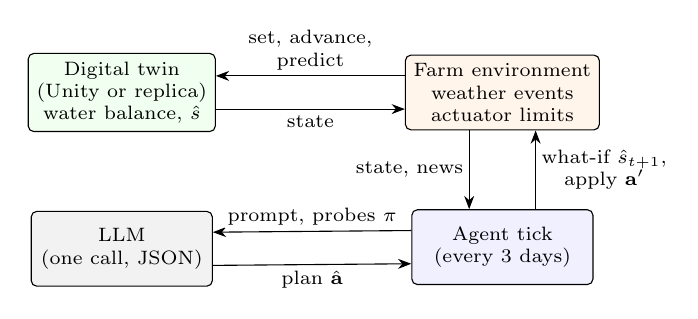
\begin{tikzpicture}[font=\scriptsize, >=Stealth, node distance=1.0cm and 2.4cm,
  box/.style={draw, rounded corners=2pt, align=center, inner sep=3pt, minimum width=2.3cm,
              minimum height=0.95cm, fill=#1},
  lab/.style={fill=white, inner sep=1pt, align=center}]
\node[box=green!6] (twin) {Digital twin\\(Unity or replica)\\water balance, $\hat s$};
\node[box=orange!8, right=of twin] (env) {Farm environment\\weather events\\actuator limits};
\node[box=blue!6, below=of env] (agent) {Agent tick\\(every 3 days)};
\node[box=gray!10, below=of twin] (llm) {LLM\\(one call, JSON)};
\draw[->] ([yshift=6pt]env.west) -- node[lab, above=1pt]{set, advance,\\predict} ([yshift=6pt]twin.east);
\draw[->] ([yshift=-6pt]twin.east) -- node[lab, below=1pt]{state} ([yshift=-6pt]env.west);
\draw[->] ([xshift=-12pt]env.south) -- node[lab, left=1pt]{state, news} ([xshift=-12pt]agent.north);
\draw[->] ([xshift=12pt]agent.north) -- node[lab, right=1pt]{what-if $\hat s_{t+1}$,\\apply $\mathbf a'$} ([xshift=12pt]env.south);
\draw[->] ([yshift=6pt]agent.west) -- node[lab, above=1pt]{prompt, probes $\pi$} ([yshift=6pt]llm.east);
\draw[->] ([yshift=-6pt]llm.east) -- node[lab, below=1pt]{plan $\hat{\mathbf a}$} ([yshift=-6pt]agent.west);
\end{tikzpicture}
\caption{One agent tick. The twin is queried before the LLM call (probes) and after it (check
of each action); only actions that pass are applied through the actuator-limited environment.}
\label{fig:arch}
\end{figure}

\textit{Control problem.} The agent can change four controls,
$\mathbf u=(\theta,\mathrm{pH},n,RH)$: irrigation or drainage, lime or sulfur, grow lights or shade
netting, and misting or ventilation. Temperature and rainfall are weather; scenarios drive them
and the agent can only compensate. Each control $j$ moves at most $\delta_j$ per action
($\delta=(20,\,0.5,\,3\,\text{h},\,15)$), so the reachable set at tick $t$ is
\begin{equation}
\mathcal A_t^j=\bigl[\max(l_j,u_t^j-\delta_j),\ \min(u_j,u_t^j+\delta_j)\bigr].
\label{eq:reach}
\end{equation}
The goals, in order, are to keep the crop alive, to reach maturity quickly and to use few
actions. The agent decides every $\tau=3$ simulated days and may change at most two controls.

\textit{Observation and prompt.} The user message is a compact JSON document (under
1{,}000 tokens with the system prompt): day, growth score, progress, stage, soil moisture, crop water use, the forecast with its
90\% range, the current weather and any event news, the name of the currently limiting variable
(the $\arg\min_j\phi_j$ if it is below 0.85, without its range), the value and reachable interval
$\mathcal A_t^j$ of every control, and the last three decisions with their observed score change.
The optimal bands $[a_j,b_j]$ never appear in the prompt.

\textit{Twin probes.} Before the call the agent asks the twin, for each control alone moved to
either end of its reachable interval, what tomorrow's score would be:
\begin{equation}
\pi^0=\hat s_{t+1}(\mathbf u_t),\qquad
\pi_j^{\pm}=\hat s_{t+1}\bigl(\mathbf u_t;\ u^j\leftarrow\text{end}^{\pm}(\mathcal A_t^j)\bigr).
\label{eq:probe}
\end{equation}
Each control's entry in the prompt maps its three levels (lowest reachable, current, highest
reachable) to $\pi_j^-,\pi^0,\pi_j^+$. The probes cost nine twin queries and no LLM calls; they
tell the model which direction helps without revealing the optimum, and replace the multi-turn
``simulate a change'' tool of an earlier tool-use version of the agent. Keying each score by its
level matters for a small model: in development, an unlabelled pair $[\pi_j^-,\pi_j^+]$ was
repeatedly read backwards by the 8B model, which then proposed lowering the pH of an acid soil.

\textit{Plan check.} The reply is parsed as
$\{\text{reasoning},\ \text{actions}=[(j,\hat a_j)]\}$; malformed replies, weather variables and
unknown names are discarded. Targets are clipped to $\mathcal A_t^j$ and changes smaller than
$0.05\,\delta_j$ are dropped, giving a plan $\mathbf a$. The twin compares each action, and then
what is left of the plan, with doing nothing:
\begin{equation}
\begin{aligned}
\mathbf a' &= \bigl\{(j,a_j)\in\mathbf a:\ \hat s_{t+1}(\mathbf u_t;\,u^j\leftarrow a_j)\ge\pi^0-\varepsilon\bigr\},\\
\text{apply } \mathbf a' &\iff \hat s_{t+1}(\mathbf u_t;\,\mathbf a')\ \ge\ \pi^0-\varepsilon,
\end{aligned}
\label{eq:check}
\end{equation}
with $\varepsilon=0.02$. Checking actions one at a time stops a harmful action from riding along
with a helpful one (an irrigation that masks a pH move in the wrong direction). Rejected actions
are listed in the next prompt. Any LLM failure (timeout, HTTP error,
invalid JSON) means no action for that tick, so the loop never stops because of the model.
Algorithm~\ref{alg:tick} summarises one tick.

\begin{algorithm}[t]
\caption{One agent tick}\label{alg:tick}
\small
\begin{algorithmic}[1]
\Require twin state $\mathbf x_t$, controls $\mathbf u_t$, history $\mathcal H$
\State $\pi^0,\{\pi_j^\pm\}\gets$ probes \eqref{eq:probe} \Comment{9 queries}
\State $m\gets$ \Call{Prompt}{$\mathbf x_t,\mathcal A_t,\pi,\mathcal H_{-3:}$}
\State $(\rho,\hat{\mathbf a})\gets$ \Call{LLM}{$m$}; \textbf{if} failure \textbf{then} $\hat{\mathbf a}\gets\emptyset$
\State $\mathbf a\gets\{(j,\clip(\hat a_j,\mathcal A_t^j)) : |\,\cdot-u_t^j|\ge0.05\delta_j\}$, $|\mathbf a|\le2$
\State $\mathbf a'\gets$ actions of $\mathbf a$ that pass the check \eqref{eq:check} alone
\If{$\mathbf a'\neq\emptyset$ \textbf{and} $\hat s_{t+1}(\mathbf a')\ge\pi^0-\varepsilon$}
  \State apply $\mathbf a'$ through the actuators
\EndIf
\State $\mathcal H\gets\mathcal H\cup\{(t,\mathbf a,\mathbf a\setminus\mathbf a',\hat s_t)\}$; advance $\tau$ days
\end{algorithmic}
\end{algorithm}

\textit{Deployment.} In Unity, a \texttt{SimulationServer} component exposes the twin over HTTP
(\texttt{/state}, \texttt{/environment}, \texttt{/predict}, \texttt{/advance}, \texttt{/log}); the
clock runs in real time (3\,s per day) and the agent's reasoning is shown in an on-screen log. For
evaluation the same agent drives the Python replica without waiting.

% =============================================================================
\section{Experimental Setup}\label{sec:setup}

\textit{Scenarios.} Every scenario except \emph{acid soil} starts from normal conditions:
25\,$^\circ$C, 62\% humidity, 8\,h of sunshine, 3\,mm/day of rain, pH 6.5 and 55\% soil moisture.
Events start without warning; the agent sees only their effects and a one-line news item.
Table~\ref{tab:scen} lists the five scenarios. Seed 0 is the canonical script; seeds 1--4 shift
each event by up to 3 days and scale its daily drift and rainfall by up to 15\%, and also draw
the plant offsets $o_i$. Each policy runs five seeds per scenario, for at most 120 days.

\begin{table}[t]
\centering
\caption{Weather scenarios (rain in mm/day)}
\label{tab:scen}
\footnotesize
\setlength{\tabcolsep}{3pt}
\begin{tabular}{@{}lp{6.3cm}@{}}
\toprule
Scenario & Events \\
\midrule
calm & none (control case) \\
drought & days 15--38: no rain, 36\,$^\circ$C, 10\,h sun, air dries 2\%/day \\
monsoon & days 16--46: 45\,mm/day, 92\% humidity, 4\,h sun; soil saturates \\
acid soil & starts at pH 4.4, 30\% soil moisture, 4.5\,h sun, 1\,mm/day; acid rain on day 30 (pH $-1.2$) \\
heatwave+storm & days 18--30: 41\,$^\circ$C, no rain, air dries 3\%/day; days 40--47: 32\,mm/day, 3\,h sun \\
\bottomrule
\end{tabular}
\end{table}

\begin{table*}[t]
\centering
\caption{Outcomes over five seeds per scenario: seasons that matured within 120 days, mean
daily growth score $H$, and totals over all 25 seasons (actions per season, mean reaction time
to weather events)}
\label{tab:results}
\footnotesize
\begin{tabular}{@{}lccccccccc@{}}
\toprule
& \multicolumn{5}{c}{Matured seasons / mean health $H$} & \multicolumn{4}{c}{All 25 seasons} \\
\cmidrule(lr){2-6}\cmidrule(l){7-10}
Policy & Calm & Drought & Monsoon & Acid soil & Heat+storm & Success & $H$ & Actions & React. (d) \\
\midrule
No intervention & 5/5, 0.97 & 0/5, 0.41 & 0/5, 0.40 & 0/5, 0.42 & 5/5, 0.80 & 40\% & 0.599 & 0.0 & -- \\
Rule-based & 5/5, 0.98 & 5/5, 0.89 & 5/5, 0.76 & 5/5, 0.88 & 5/5, 0.87 & 100\% & 0.877 & 10.2 & 3.5 \\
\midrule
LLM agent & 5/5, 0.98 & 5/5, 0.89 & 4/5, 0.68 & 5/5, 0.81 & 5/5, 0.86 & 96\% & 0.843 & 13.7 & 3.6 \\
Agent, no probes & 5/5, 0.97 & 5/5, 0.88 & 5/5, 0.74 & 2/5, 0.73 & 5/5, 0.85 & 88\% & 0.835 & 15.8 & 3.2 \\
Agent, no twin check & 2/5, 0.62 & 5/5, 0.78 & 3/5, 0.64 & 2/5, 0.73 & 1/5, 0.51 & 52\% & 0.657 & 40.0 & 1.0 \\
Agent, Mistral 24B & 5/5, 0.98 & 5/5, 0.91 & 4/5, 0.68 & 5/5, 0.89 & 5/5, 0.88 & 96\% & 0.869 & 11.6 & 2.3 \\
\bottomrule
\end{tabular}

\end{table*}

\begin{figure*}[t]
\centering
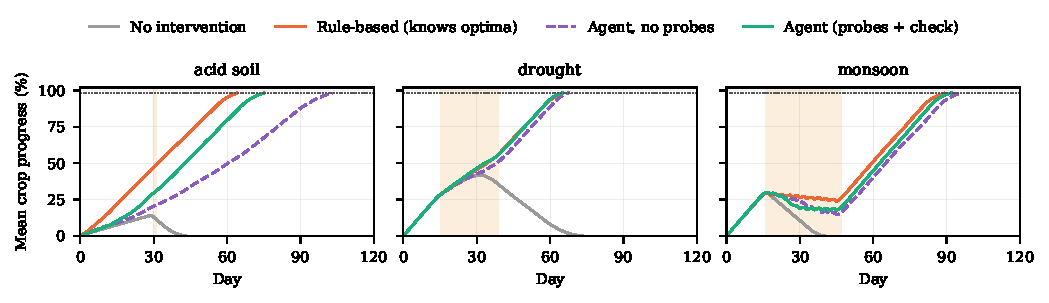
\includegraphics[width=\textwidth]{figures/progress.pdf}
\caption{Mean crop progress over the canonical season (seed 0) in three scenarios; weather
events are shaded and the dotted line marks maturity (98\%). Without intervention the crop
dies in all three; the agent's probes close most of the gap to the rule-based controller on
acid soil.}
\label{fig:progress}
\end{figure*}

\textit{Policies.} \emph{No intervention} never touches the controls. \emph{Rule-based} is a
threshold controller that knows the true optimal bands and, every three days, resets any
out-of-band control to the band centre (within the same actuator limits); it has information
the agent does not. The \emph{LLM agent} uses Llama~3.1~8B Instruct \cite{grattafiori2024llama3}
(Turbo endpoint on DeepInfra, temperature 0.2, at most 300 output tokens, JSON mode). Three
ablations change one thing each: no probes (the prompt without $\pi$), no twin check
(\eqref{eq:check} disabled), and a larger model, Mistral Small~3 (24B) \cite{mistral2025small3}.

\textit{Metrics.} A season succeeds if the field matures within 120 days. Crop health is the
mean daily score $H=\frac{1}{D}\sum_{t=1}^{D}\hat s_t$ over the $D$ simulated days. Reaction time
is the number of days from an event's onset to the first equipment action after it, counting 1
when the policy acts at the first decision that sees the event. We also count actions per
season, decisions with an action vetoed by the twin, and the cost $C=(N_{\text{in}}c_{\text{in}}+N_{\text{out}}c_{\text{out}})/10^6$ USD for
$N$ tokens at the provider's per-million prices $c$.

% =============================================================================
\section{Results}\label{sec:results}

Table~\ref{tab:results} gives the outcomes and Fig.~\ref{fig:progress} three representative
seasons.

\textit{Agent versus baselines.} Without intervention the crop dies in every drought, monsoon
and acid-soil season (40\% success). The LLM agent matures 24 of 25 seasons (96\%) with mean
health 0.843, against 100\% and 0.877 for the rule-based controller, which knows the optimal
bands the agent has to discover. The gap is concentrated where the agent must move a variable
far from its start: on acid soil it matures in 86 days on average versus 68 for the rule,
since it takes longer to bring pH, light and soil moisture into range, and several of its pH
moves are vetoed along the way. In the drought the agent matches the rule (0.891 versus 0.890
health, 66.4 versus 66.6 days to maturity) and reacts twice as fast (3.4 versus 7.0 days), since
it does not wait for a variable to leave its optimal band before acting. The agent uses 13.7 actions per season against the rule's 10.2.

\textit{Ablations.} Removing the twin check is catastrophic: success falls to 52\%, health to
0.657, and actions almost triple (40 per season). The unchecked 8B model reacts fastest
(1.0 days) but often in the wrong direction, and it loses three of five \emph{calm}
seasons, where doing nothing would have been perfect. With the check, the 8B model has 13.9 plans
per season partly or wholly vetoed, more than half of its 25.8 decisions: it is a noisy
proposer, and the twin turns it into a safe one. Removing the probes lowers success to 88\%:
acid soil drops from 5/5 to 2/5 and its maturity from 86 to 108 days, because, told only that pH
is limiting, the model often lowers it (Section~\ref{sec:agent}). The probes cost nine twin
queries per decision and about 100 extra prompt tokens. Replacing the 8B model by Mistral Small~3
(24B) keeps 96\% success but raises health to 0.869, shortens mean maturity over matured
seasons from 74.7 to 68.8 days (rule: 70.4), uses fewer actions (11.6) and needs only 3.5 vetoes per season.

\begin{table}[t]
\centering
\caption{Agent behaviour per season (means over 25 seasons)}
\label{tab:agent}
\scriptsize
\setlength{\tabcolsep}{2.5pt}
\begin{tabular}{@{}lcccccc@{}}
\toprule
Variant & Calls & Vetoed & Errors & Tokens/call & Latency (s) & USD \\
\midrule
LLM agent & 25.8 & 13.9 & 4.0\% & 897 & 3.75 & 0.00055 \\
no probes & 28.8 & 15.7 & 3.9\% & 791 & 3.07 & 0.00055 \\
no twin check & 32.8 & 0.0 & 2.3\% & 883 & 3.00 & 0.00068 \\
Mistral 24B & 23.9 & 3.5 & 0.7\% & 981 & 2.33 & 0.00129 \\
\bottomrule
\end{tabular}

\end{table}

\textit{Cost and reliability.} Table~\ref{tab:agent} lists the LLM usage. A season takes 24--33
calls of about 900 prompt tokens (system prompt included) and costs \$0.00055 with the 8B model
and \$0.0013 with the 24B model; all 100 agent seasons in this study cost \$0.077. Of about 2{,}800
calls, six failed on the network; the other flagged replies tried to set temperature (a weather
variable) or proposed more than two actions, and were trimmed or ignored by validation. No reply
crashed the loop.

\textit{Failure case.} Both probe-guided agents lose the same season: monsoon seed~2, whose
jittered rain (51\,mm/day) keeps the soil saturated whatever drainage is applied. Both
models keep draining the soil, which the check accepts but which cannot help, and neglect humidity
and light, whose single-day effect is below $\varepsilon$. The rule-based controller fixes all
three, slows the decline slightly, and survives the event with 4\% progress left.

% =============================================================================
\section{Discussion and Limitations}

\textit{Division of labour.} The results suggest a split between the components. The LLM supplies
priors and initiative: it knows that dry air and heat call for misting and irrigation, reacts
at the first sign of an event, and needs no optimal ranges. The twin supplies grounding: it
tells the model which direction helps and refuses actions that it predicts would hurt. Neither
is enough alone. The twin without a proposer does nothing, and the proposer without the twin
does worse than no management on calm and heatwave seasons. This mirrors SayCan's
language-times-affordance decomposition \cite{ahn2022saycan} and RAP's planning with a world
model \cite{hao2023reasoning}, at a far smaller scale and cost. A larger model mostly
reduces the vetoes, so the check matters most for the cheapest models. The monsoon failure
shows the limit of a one-step check: it cannot value actions whose benefit is small per day
but accumulates, and a multi-day rollout of the twin over the decision interval is the natural
next step.

\textit{Limitations.} The field is simulated: the process model uses tomato-like cardinal
ranges and FAO-56 coefficients rather than measurements from a real plot, and the agent is
evaluated against the same surrogate it queries, so the probes are exact by construction. With
a physical farm the twin would carry model error, and the conformal band would need to enter
the check. The check looks one day ahead; plans whose benefit appears only later (draining
before forecast rain, gradual liming) are judged by their first day. Five seeds per scenario
and a stochastic LLM give wide intervals for single scenarios. Finally, the rule-based
baseline is an upper reference rather than a competitor: it is given the true optima.

% =============================================================================
\section{Conclusion}

We presented a twin-in-the-loop farm manager in which a small open language model proposes
actions and a learned plant-growth digital twin probes and checks them. On a benchmark of five
weather scenarios, an 8B model guided this way brings 96\% of seasons to maturity for well
under a tenth of a cent per season, close to a rule-based controller that is given the true
optima, while the same model without the twin check succeeds in only 52\%. Future work will add
multi-day rollouts and the conformal band to the check, and evaluate the agent on a twin
calibrated to a real field.

\bibliographystyle{IEEEtran}
\bibliography{refs}

\end{document}
